\chapter{Przegląd istniejących rozwiązań}
	Procesor Zilog Z80 dorobił się wielu emulatorów, pisanych kiedyś przez duże firmy, a aktualnie przez hobbystów. Na popularnej usłudze hostingowej Github przeznaczonej dla projektów programistycznych, można znaleźć około 200 repozytoriów z projektami emulującymi Z80, lub emulującymi urządzenia używające tego procesora, co dowodzi jego popularności.\cite{githubZ80Emulators}   
	
	 Poniżej prezentuje najciekawsze pozycje tych programów, które posiadają graficzny interfejs użytkownika, i pozwalają na wgląd w  wewnętrzne stany procesora. Przedstawię zarówno komercyjne rozwiązania, jak i te pisane przez amatorów.
	
	\section{Z80 SIMULATOR IDE}
	Dostępny pod adresem http://www.oshonsoft.com/z80.html płatny symulator posiadający najbardziej rozbudowany interfejs z wszystkich wymienionych pozycji. Pozwala on na prezentowanie wewnętrznych stanów procesora, manipulacją przerwaniami, edytor pamięci umożliwiający działający również podczas symulacji, podgląd i manipulacja portami wejścia/wyjścia. Posiada również funkcje typowe dla debuggerów, możliwość wstrzymania działania programu w określonym miejscu, tryb pracy krokowej, interaktywny edytor i kompilator kodu asemblera.\cite{oshonsoftEmulator} Część funkcji została zaprezentowana na rysunku \ref{img:oshonsoftEmulator} 
	
	\begin{figure}[h]
		\centering
		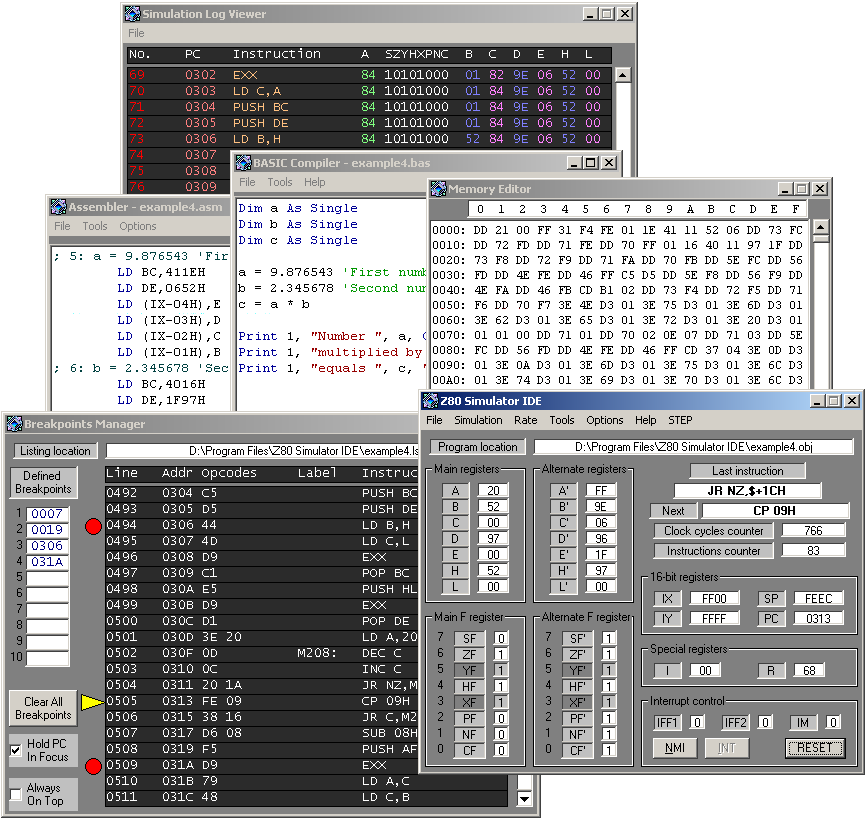
\includegraphics[width=0.7\textwidth]{oshonsoftEmulator}
		\caption{Z80 SIMULATOR IDE \cite{oshonsoftEmulator}}
		\label{img:oshonsoftEmulator}
	\end{figure}
	
	Do wad emulatora należy interfejs, który nie jest intuicyjny. Dla przykładu, w żadnym miejscu nie znajdziemy informacji, o tym w jakim formacie powinny być wprowadzane wartości liczbowe. Brak w programie systemu pomocy, opisów, co może odstraszyć początkującego użytkownika. Dodatkowo jest to rozwiązanie płatne i przeznaczone tylko dla platformy MS Windows. Jest to narzędzie głównie dla specjalistów.
	
	
	\section{ZEMU - Z80 Emulator Joe Moore}
	Jest to emulator zaprojektowany głównie, dla uruchamiania systemu CPM. Była to seria systemów operacyjnych oferowana przez firmę Digital Research Inc i latach 1970-1980.\cite{cpm}
	
	Program skierowany jest do hobbystów. Oprócz standardowych możliwości takich jak podgląd i edycja pamięci, rejestrów, flag ma możliwość emulacji stacji dyskietek, portu COM, portu szeregowego, monitora CRT, drukarki.    
	
	Na rysunku \ref{img:zemu} przedstawiono interfejs aplikacji. Tak jak w przypadku Z80 SIMULATOR IDE jest on nie intuicyjny, brak mu systemu pomocy, elementy interfejsu nie są opisane w wystarczającym stopniu. Osoby nie mające doświadczenia z urządzeniami wejścia wyjścia w Zilogu Z80 będą miały problem z obsługą nawet podstawowych funkcji.
	
	Inną wadą aplikacji jest możliwość jej uruchomienia tylko w systemie Windows. 
	
	\begin{figure}[h]		
		\centering
		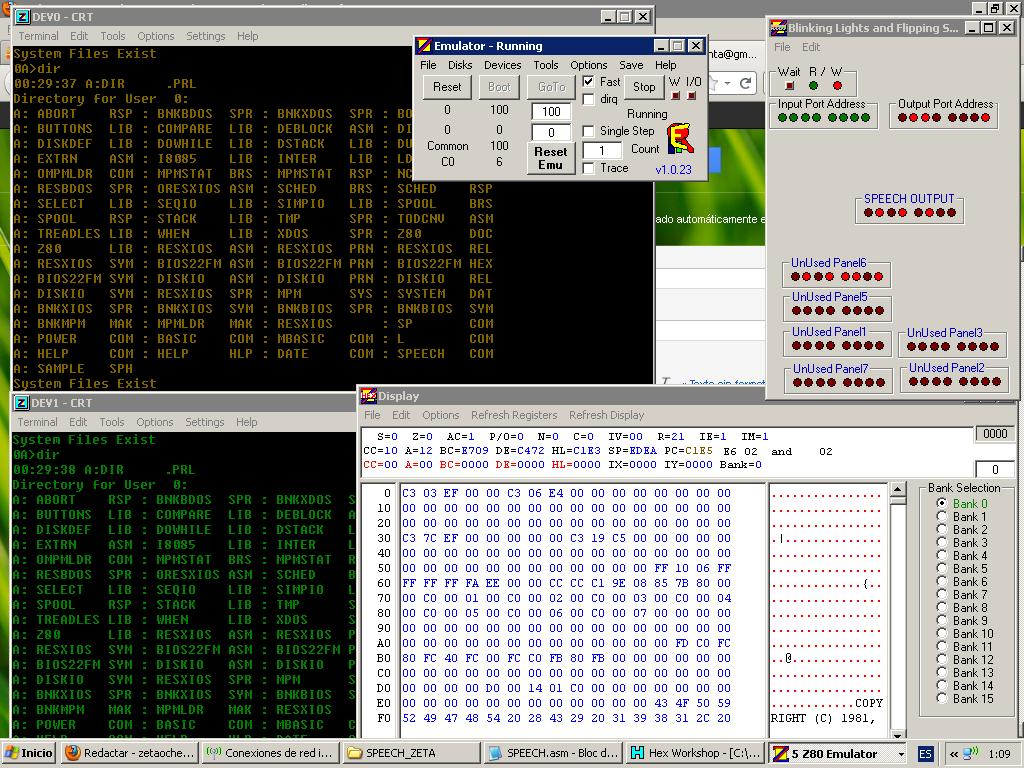
\includegraphics[width=0.8\textwidth]{zemu}
		\caption{ZEMU \cite{zemuImg}}
		\label{img:zemu}
	\end{figure}
	
	 \section{ZIM - The Z80 Machine Simulator}
	ZIM został napisany za pomocą technologi Java Web-Start. Pozwala to na uruchomienie aplikacji bezpośrednio na stronie internetowej, wraz z dostępem do lokalnych zasobów systemu, np plików. \cite{zim}
	Aplikacja według autora \cite{zimPurpose} przeznaczona jest głównie dla studentów uczących się języka asemblera dla procesora Z80.
	
	Aplikacja pozwala podgląd wszystkich wewnętrznych parametrów cpu, podłączać proste urządzenia wejścia wyjścia, edytować pamięć, debugować program, symulować przerwania. Zaletą programu jest jego wieloplatformowość dzięki zastosowaniu języka Java.
	
	Brakuje w niej natomiast edytora asemblera, systemu pomocy, interfejs ma wiele błędów i nie jest intuicyjny. Na rysunku \ref{img:zim} przedstawiono zrzut ekranu działającej aplikacji.
	
	\begin{figure}[h]		
		\centering
		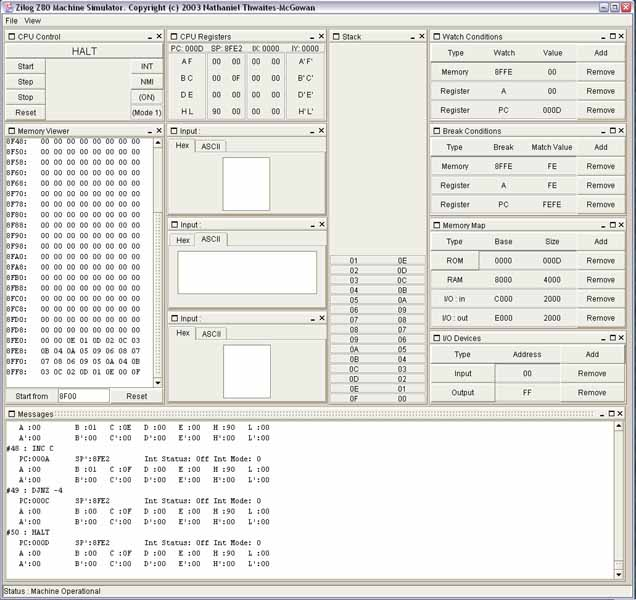
\includegraphics[width=0.8\textwidth]{zim}
		\caption{ZIM - The Z80 Machine Simulator \cite{zimImg}}
		\label{img:zim}
	\end{figure}
	
	%Żadne istniejące rozwiązanie nie pozwala na podejrzenie wewnętrznych magistrali procesora
	
	\section{Podsumowanie istniejących rozwiązań}
	Problemem prawie wszystkich emulatorów i symulatorów jest interfejs. Nie tyczy się to konkretnie omawianego procesora, ale ogółu tego typu aplikacji. Są one przeznaczone dla osób znających architekturę komputerową, oraz budowę i działanie konkretnego emulowanego urządzenia, dlatego programiści nie przywiązują do intuicyjności i systemów pomocy odpowiedniej wagi. Osoby nie posiadające wymaganej wiedzy, albo znające jedynie podstawy nie są w stanie sprawnie obsługiwać programu. 
	
	Emulatory rzadko są wielkoformatowe. Dotyczy się to szczególnie aplikacji emulujących przez re-kompilacje. Aby ją wykonać wymagana jest znajomość architektur wyjściowej i docelowej. Rozwiązaniem tego problemu mogą być interpretery napisane w języku Java, tak jak "ZIM - The Z80 Machine Simulator". Rozwiązanie to jest wolne, kod emulowanej architektury jest najpierw interpretowany przez interpreter napisany w języku Java, a następnie ponownie emulowany już przez dynamiczną re-kompilacje w maszynie wirtualnej. Typowe rozwiązania napisane w języku kompilowanym pod konkretny procesor działają szybciej, kosztem wieloplatformowość. Optymalizacja w sprzęcie typu Zilog Z80 nie jest kluczową kwestią, współczesne komputery są na tyle szybkie, aby uruchomić emulator maszyny z lat 70 napisanej w Javie. 
	
	Kolejną kwestią o której warto wspomnieć jest czytelność kodu. Kod istniejących rozwiązań nie należy do przejrzystych, najczęściej cały kod emulatora zawiera się w jednym pliku z kilkuset liniami. Osoba pragnąca wgłębić się w sam proces emulacji w takim przypadku ma utrudnione zadanie.
	
	Podsumowując, aktualnie brakuje wieloplatformowego emulatora lub symulatora Ziloga Z80, z czytelnym, poprawnie działającym interfejsem, przejrzystym dobrze komentowanym kodem źródłowym, i system pomocy.
	
	